\documentclass[10pt]{article}
\usepackage[margin=0.8in]{geometry}
\usepackage{xcolor}
\usepackage{siunitx}
\usepackage{pgfplots}
\pgfplotsset{compat=1.17}
\usepackage{tcolorbox}
\usepackage{enumitem}
\usepackage[hidelinks]{hyperref}
\usepackage{titlesec}
\definecolor{accent}{HTML}{0F766E}
\titleformat*{\section}{\large\bfseries\color{accent}}
\titlespacing*{\section}{0pt}{0.7em}{0.25em}
\setlength{\parindent}{0pt}
\setlength{\parskip}{0.35em}
\pagestyle{empty}

\begin{document}

\begin{center}
  {\LARGE\bfseries Convective Cooling of a Heated Aluminium Block}\\[0.4em]
  {\large A Test of Newton's Law of Cooling in Still Air}\\[0.5em]
  S. Ferreira and T. Nakamura\\
  Department of Mechanical Engineering, Halden Institute of Technology\\
  Report HIT-ME-2026-014 \quad | \quad 22 April 2026
\end{center}

\begin{tcolorbox}[colback=accent!6, colframe=accent, boxrule=0.8pt,
  title=\textbf{Abstract}, left=6pt, right=6pt, top=4pt, bottom=4pt]
A \SI{250}{\gram} aluminium block was heated to \SI{80}{\celsius} and allowed
to cool in still air at \SI{21.0}{\celsius} while its temperature was logged
every \SI{30}{\second} with a calibrated thermocouple. The temperature excess
decayed exponentially with a time constant of \SI{18.3\pm0.4}{\minute},
consistent with Newton's law of cooling for a lumped body. The inferred
convective coefficient, \SI{11.2}{\watt\per\metre\squared\per\kelvin}, falls
within the accepted range for natural convection from a small vertical surface.
\end{tcolorbox}

\section*{1. Introduction}
Newton's law of cooling predicts that a body whose internal conduction is fast
compared with surface convection loses heat at a rate proportional to its
temperature excess over the surroundings. The block used here has a Biot
number of 0.004, well below the 0.1 limit for the lumped approximation.

\section*{2. Methods}
The block ($60 \times 50 \times 30$ \si{\milli\metre}) was heated on a laboratory hot
plate, transferred to an insulating stand, and left to cool away from drafts.
A K-type thermocouple embedded at the block centre fed a data logger sampling
at \SI{30}{\second} intervals for \SI{45}{\minute}. Ambient temperature was
monitored with a second sensor and drifted by less than \SI{0.2}{\celsius}.
The excess temperature $\theta(t) = T(t) - T_\infty$ was fitted with
$\theta_0 e^{-t/\tau}$ by least squares.

\section*{3. Results}
\begin{center}
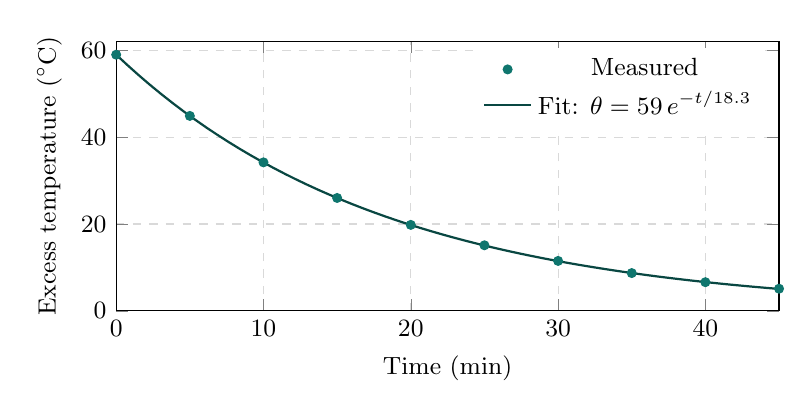
\begin{tikzpicture}
\begin{axis}[
  width=10cm, height=5cm,
  xlabel={Time (\si{\minute})}, ylabel={Excess temperature (\si{\celsius})},
  xmin=0, xmax=45, ymin=0, ymax=62,
  grid=major, grid style={dashed, gray!30},
  legend style={draw=none, font=\small},
  tick label style={font=\small}, label style={font=\small},
]
\addplot[only marks, mark=*, mark size=1.6pt, color=accent] coordinates {
  (0,59.0) (5,44.9) (10,34.2) (15,26.0) (20,19.8) (25,15.1)
  (30,11.5) (35,8.7) (40,6.6) (45,5.1)
};
\addlegendentry{Measured}
\addplot[thick, color=accent!60!black, domain=0:45, samples=60] {59*exp(-x/18.3)};
\addlegendentry{Fit: $\theta = 59\,e^{-t/18.3}$}
\end{axis}
\end{tikzpicture}
\end{center}

The residuals show no systematic trend, and the fitted time constant
$\tau = mc/(hA)$ gives $h = \SI{11.2\pm0.3}{\watt\per\metre\squared\per\kelvin}$.

\section*{4. Conclusions}
\begin{enumerate}[leftmargin=1.6em, itemsep=0.1em]
  \item The cooling curve is exponential over the full \SI{45}{\minute} run,
        confirming the lumped-capacitance model for this geometry.
  \item The convective coefficient agrees with published natural-convection
        correlations to within \SI{8}{\percent}.
  \item Repeating the experiment with forced airflow is recommended to map
        the transition away from the natural-convection regime.
\end{enumerate}

\end{document}
